%!TEX program = xelatex
\documentclass[tikz, border=5pt]{standalone}  % 核心修改:启用独立画布
\usepackage[dvipsnames]{xcolor}
\usepackage{pgfplots}
\usepgfplotslibrary{colormaps}
\pgfplotsset{compat=1.18}

\begin{document}
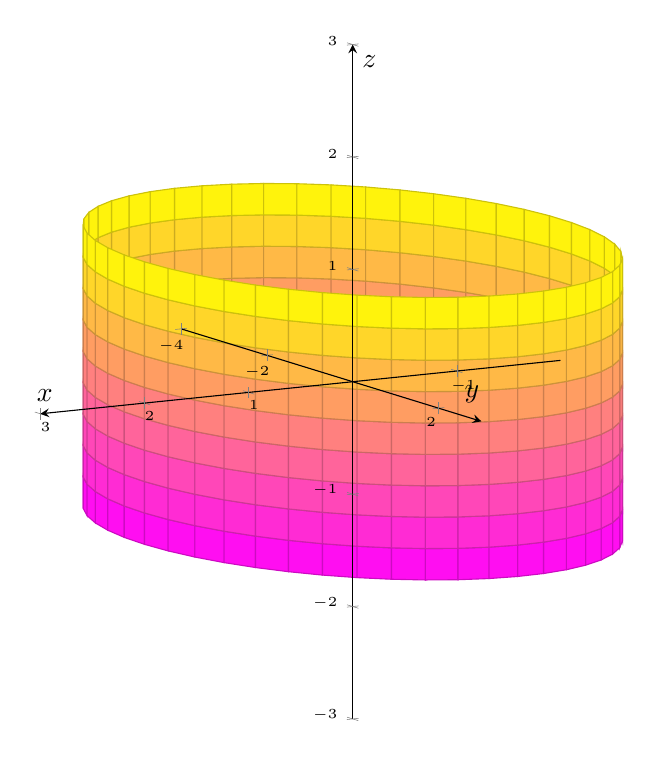
\begin{tikzpicture}
    \begin{axis}[
        tick label style={font=\tiny},
        view={150}{9},
        axis lines=center,
        axis on top,
        xlabel={$x$}, ylabel={$y$}, zlabel={$z$},
        xmax=3, ymax=3, zmax=3, zmin=-3,
        width=12cm, height=12cm,
        colormap/spring  % 修正色彩映射声明位置
    ]
        \addplot3 [
            surf,
            z buffer=sort,
            samples=50,
            samples y=10,       % 优化y方向采样率
            domain=0:2*pi,
            y domain=-0.4*pi:0.4*pi
        ] ({2*cos(deg(x))},{4*sin(deg(x))},{y});
    \end{axis}
\end{tikzpicture}
\end{document}
